\documentclass[a4paper, 10pt]{report}
\usepackage[italian]{babel}
\usepackage[T1]{fontenc}
\usepackage[utf8]{inputenc}
\usepackage{charter}
\usepackage{amsmath}
\usepackage{amsthm}
\usepackage{amsfonts}
\usepackage{graphicx}
\usepackage{wrapfig}
\usepackage{tcolorbox}
\usepackage{fancyhdr}
\usepackage{listings}

\usepackage{geometry}
\geometry{a4paper, left=2cm,right=2cm,top=2cm,bottom=2cm}

\pagestyle{fancy}
\lhead{}
\chead{}
\rhead{\bfseries 24 ottobre 2019 }
\lhead{\bfseries Linguaggi}

\begin{document}

\subsection*{Semantica delle espressioni}
La sintassi delle espressioni è la seguente:
\lstset{language=C}
\begin{lstlisting}
<Exp>
E -> A | B
A -> I | N | A op B
B -> true | false | not B | B bop B
\end{lstlisting}

\noindent dove:
\begin{itemize}
\item[-] A e B indicano rispettivamente espressioni aritmetiche e booleane;
\item[-] L'inseme op indica le operazioni {+, -, *};
\item[-] L'inseme bop indica le operazioni {or, =}.
\end{itemize}

\paragraph*{Rappresentazione} Le metaviariabili sono le seguenti:
\begin{itemize}
\item[-] Espressioni $\varepsilon$: $e$
\item[-] Numeri $N$: n, m, p
\item[-] Booleani $B$: $t$
\end{itemize}

\paragraph*{Valutazione} La valutazione delle espressioni è una funzione $Eval: \varepsilon \rightarrow N \cup B$ che descrive il comportamento dinamico delle espressioni restituendo il valore in cui esse sono valutate:
\begin{align*}
(Eval(e) = k) \longleftrightarrow (e \rightarrow^* k)
\end{align*}

\paragraph*{Equivalenza}L'equivalenza di espressioni è una realzione $\equiv \subseteq \varepsilon x \varepsilon$   definita come:
\begin{align*}
(e_1 \equiv e_2) \longrightarrow (Eval(e_1) = Eval(e_2))
\end{align*}

\subsection*{Regole}

\begin{center}
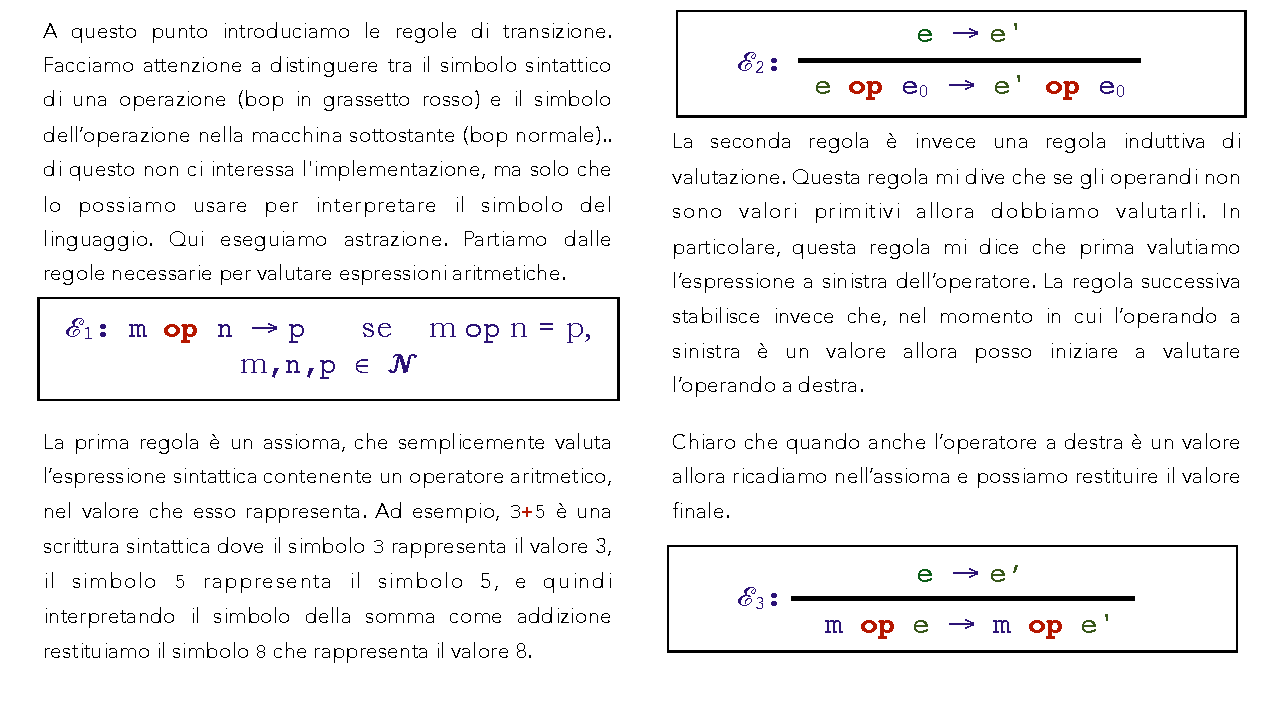
\includegraphics[scale=0.8]{exp1.pdf}

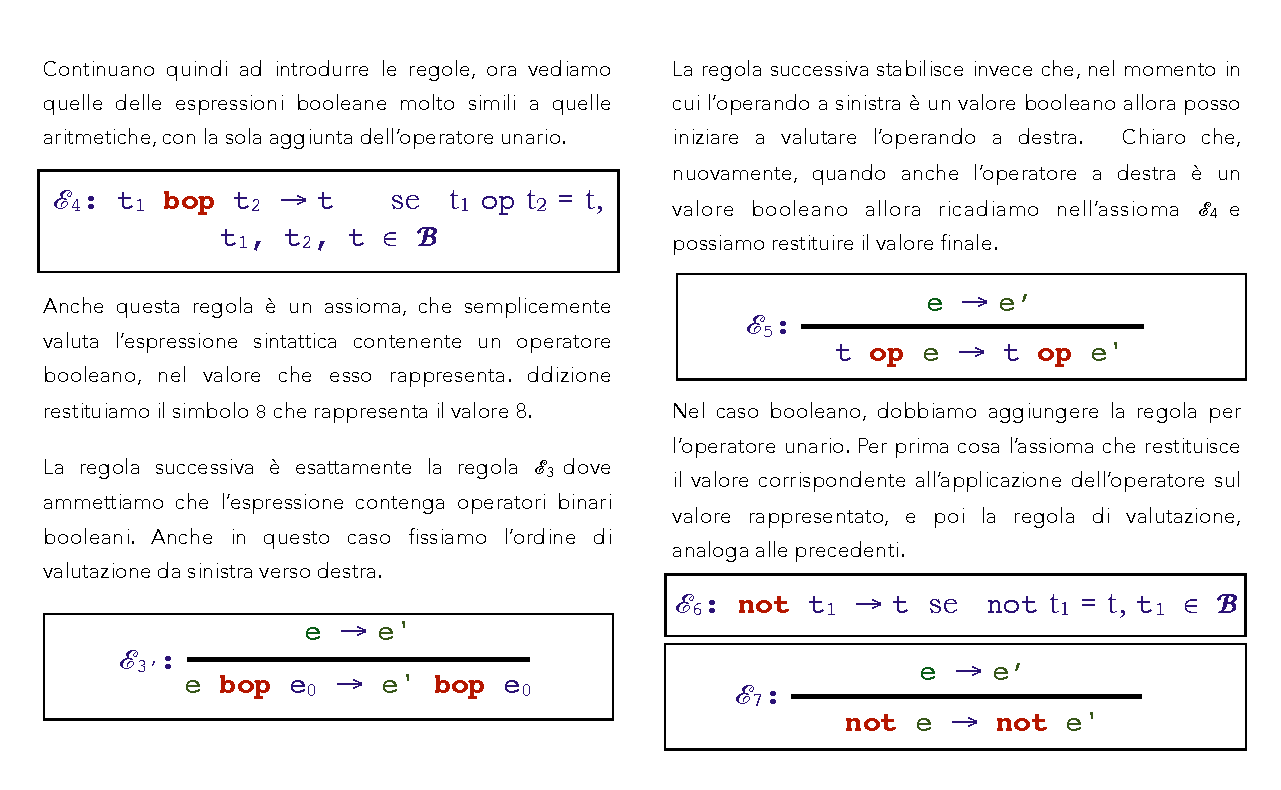
\includegraphics[scale=0.8]{exp2.pdf}
\end{center}

\noindent \underline{Esempio di applicazione delle regole}:

\begin{align*}
(2 + 3) * (5 - (1 + 4))
\end{align*}

\noindent Poichè l'operatore $*$ non ha numeri ne a destra ne a sinistra non è possibile applicare la regola $\varepsilon_1$. Applico quindi le altre due regole:\\

Applico la regola $\varepsilon_2$:
\begin{align*}
\frac{2 + 3 \rightarrow 5}{(2+3)*(5-(1+4)) \rightarrow 5*(5-(1+4))}
\end{align*}

Applico la regola $\varepsilon_3$:
\begin{align*}
\frac{\frac{1+4 \rightarrow 5}{5-(1+4) \rightarrow 5 - 5}}{5*(5-(1+4)) \rightarrow 5*5-5}
\end{align*}

Applico la regola $\varepsilon_3$:
\begin{align*}
\frac{5 - 5 \rightarrow 0}{5*5-5 \rightarrow 5*0}
\end{align*}

\begin{center}
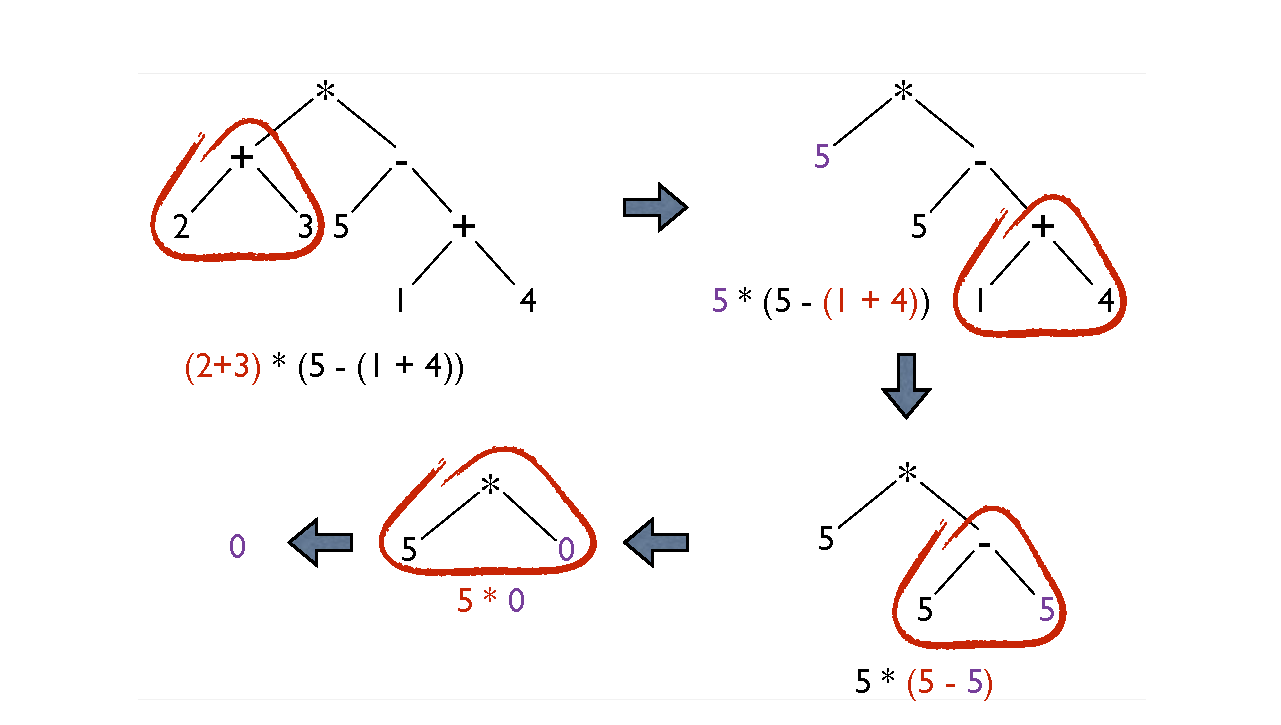
\includegraphics[scale=0.8]{esempio1.pdf}
\end{center}

\noindent In gran parte dei linguaggi le espressioni devono essere risolte da destra verso sinistra. In specifici linguaggi è possibile anche il contrario (non nel nostro caso).\\

\paragraph*{Valutazione delle espressioni} La valutazione delle espressioni è una funzione $Eval: \varepsilon \rightarrow N \cup B$ (numeri unito a booleani) ce descrive il comportamento dinamico delle espressioni restituendo il valore in cui esse sono valutate:
\begin{align*}
(Eval(e) = k) \longleftrightarrow (e \rightarrow^* k)
\end{align*}

\paragraph*{Equivalenza di espressioni} L'equivaleza di espressioni è una relazione $\equiv \subseteq \varepsilon x \varepsilon$ definita come segue:
\begin{align*}
(e_0 \equiv e_1) \longleftrightarrow (Eval(e_0) = Eval(e_1))
\end{align*}
Quindi due espressioni sintatticamente diverse sono uguali quando rappresentano lo stesso valore (hanno lo stesso significato).

\section*{\underline{Dichiarazioni}}
Le dichiarazioni sono la categoria sintattica che crea e modifica gli ambienti. Le dichiarazioni devono essere elaborate affinchè possano operare. 

Le modifiche effettuate sono reversibili, in quanto valide solo all'interno dello scope dell'identificatore. Quindi è possibile avere più identificatori con lo stesso nome. Possono evere side-effects.

\subsection*{Identificatori}
Un indentificatore è una string adi caratteri usata per denotare "altro". 
Un identificatore può denotare più elementi, mentre un elemento può essere denotato da più identificatori diversi (aliasing).\\

\noindent A seconda del linguaggio, la scelta del nome dell'identificatore può essere vincolato a delle regole:
\begin{itemize}
\item[-] Utilizzo del case-sensitive;
\item[-] Presenza di parole riservate;
\item[-] Possibili vincoli di lunghezza;
\item[-] Vincolo nella presenza di caratteri speciali.
\end{itemize}

\paragraph*{Rappresentazione} Identificatori $Id$: $id, x$.

\subsection*{Bindings}
Il concetto di bindings viene ereditato dalla matematica.
Per prima cosa si dichiarano l'identificatore e il suo significato, ovvero si crea il legame nelle occerrenze di bindings (tipo "sia x qualcosa" in matematica):
\begin{center}
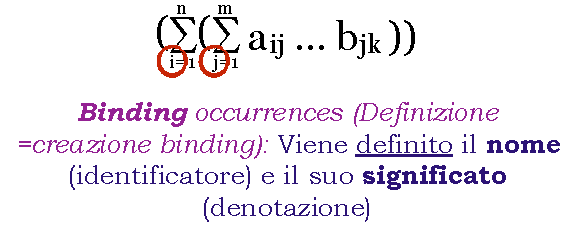
\includegraphics[scale=0.7]{1.pdf}
\end{center}

\noindent Se il nome è associato ad un significato, allora ogni sua occorrenza è un'occorrenza applicata:
\begin{center}
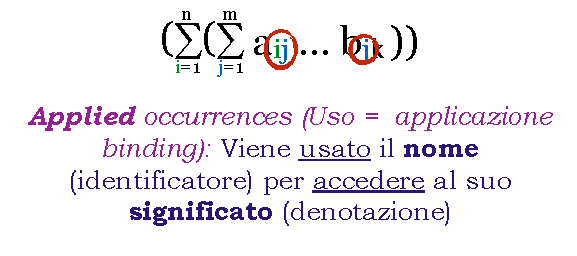
\includegraphics[scale=0.7]{2.pdf}

\end{center}

\noindent Se non viene definito il significato dell'identificatore, allora ogni sua occorrenza è un'occorrenza libera (può rappresentare qualunque cosa):
\begin{center}
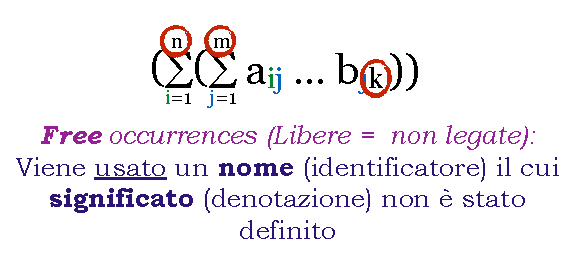
\includegraphics[scale=0.7]{3.pdf}

\end{center}

\noindent La differenze tra occorrenze libere e applicate consiste nel raggio di azione dell'occorrenze 
\begin{center}
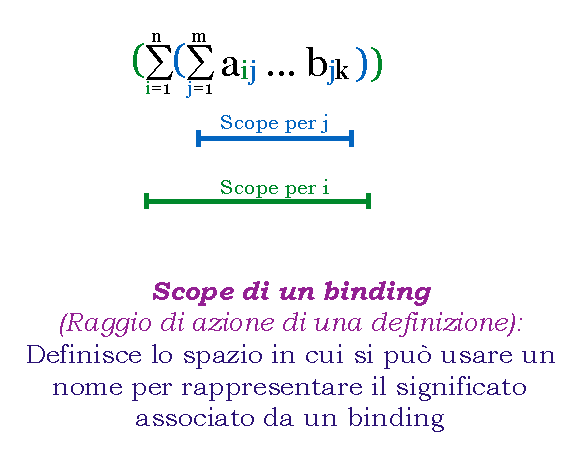
\includegraphics[scale=0.7]{4.pdf}

\end{center}

\noindent Esistono quindi tre possibili tipo di occorrenza di un identificatore:
\begin{itemize}
\item[-] Occorrenza di definizione (binding occurence), che si ha quando si definisce (o ridefinisce) il significato dell'identificatore;
\item[-] Occorrenza applicata, che si ha quando si utilizza l'identificatore per riferirsi al suo significato;
\item[-] Occerrenza libera, che si ha quando l'identificatore non si trova nello scope della sua definizione.
\end{itemize}

\paragraph*{Tipi di bindings} Esistono due tipi di bindings:
\begin{itemize}
\item[-] Binding statico -> il legame non può variare durante l'esecuzione (es: tipo di una variabile);
\item[-] Binding dinamico -> il legame può variare durante l'esecuzione
\end{itemize}

















\end{document}